\documentclass{cmc}

\hypersetup{ colorlinks=true, linkcolor=blue, filecolor=magenta, urlcolor=red, }
\urlstyle{same}

\title{Instructions for using Git}

\begin{document}

\maketitle
\tableofcontents
\pagestyle{fancy}
\lhead{\textit{\textbf{Computational Motor Control, Spring 2019} \\
    Git Tutorial, Lab 0, NOT GRADED}} \rhead{Student \\ Names}

\newpage

\section{GIT}
\label{sec:git}

This document outlines the basic steps to clone and stay up to date
with the CMC-2019 exercises using Git. It is not a comprehensive
tutorial on using Git. For detailed tutorials please use the
references below.

\begin{itemize}
\item \href{http://ndpsoftware.com/git-cheatsheet.html}{Git
    Cheat sheet}
\item \href{https://learngitbranching.js.org}{Interactive tutorial}
\item \href{https://try.github.io/levels/1/challenges/1}{Try Git!}
\item
  \href{https://marklodato.github.io/visual-git-guide/index-en.html}{A
    Visual Git Reference}
\item \href{http://rogerdudler.github.io/git-guide/}{git-guide}
\end{itemize}


\section{Authorization}
In order to pull or push the git repository you need to first set a
password to your account.  To do this, on your default browser login
to the following URL with your epfl credentials.

\url{https://gitlab.epfl.ch/BioRobCMC/2019}

Once you open the page, you should see a banner that looks the image
below.

\begin{figure}[h]
  \centering 
\includegraphics[width =
  \textwidth]{figures/GitAuthorization}
  \caption{HTTPS Git Authorization}
  \label{fig:authorization}
\end{figure}

Click on the set password and create the password. \textbf{It is
  important that you do this step in order to clone the repository.}

If you do not see this then you have probably already authorized your
account.

\section{Windows}
\label{sec:windows}

\subsection{Cloning}
\label{sec:windows_cloning}
\begin{itemize}
\item If you haven't already then download the Git Bash application
  from \href{https://git-scm.com/download/win}{Git}

  \textbf{Note:} During installation, choose \textit{Use Git from Git
    bash only}

\item After installation, either from the main menu or on your Desktop
  you should now find Git Bash application
\item Open Git Bash
\item Navigate to the location where you want to install the CMC
  exercises folder. For example, if you want to navigate to your
  Desktop:

  \begin{center}
    \$ cd \verb|C:/Users/(YOUR_USER_NAME)/Desktop|
  \end{center}

\item Then execute the following command to clone the repository:
  \begin{center}
    \$ git clone \verb|https://gitlab.epfl.ch/BioRobCMC/2019.git|
  \end{center}

  This would clone the repository with the default folder name
  \verb|2019|. If you wish to clone with a different folder name, then
  use the following command and replace \verb|FOLDER_NAME| with the
  name of the folder you want to clone into:
  \begin{center}
    \$ git clone \verb|https://gitlab.epfl.ch/BioRobCMC/2019.git|
    \verb|FOLDER_NAME|
  \end{center}

\end{itemize}

\subsection{Pulling}
\label{sec:windows_pulling}

In order to stay up to date with the changes made in the repository,
you will have to do a git pull to get the latest version of the
exercises.

\begin{itemize}
\item Open Git Bash
\item Navigate to the exercise directory (Like you did while cloning!)
  \textbf{NOTE : } You need to be anywhere inside the repository
  directory!!
\item Execute the following command:
  \begin{center}
    \$ git pull origin master
  \end{center}
\end{itemize}

If you have the latest version then the output of the above command
should be:

\begin{center}
  \$ Already up-to-date!
\end{center}

Since this is a public repository for all students, you can not push
your changes to the repository.


\section{MacOS}
\label{sec:macos}

\subsection{Cloning}
\label{sec:macos_cloning}
\begin{itemize}
\item Open Terminal using Spotlight search. You can also go to
  Applications -> Utilities -> Terminal
\item Navigate to the location where you want to install the CMC
  exercises folder. For example, if you want to navigate to your
  Desktop:

  \begin{center}
    \$ cd \verb|~/Desktop|
  \end{center}

\item Then execute the following command to clone the repository:
  \begin{center}
    \$ git clone \verb|https://gitlab.epfl.ch/BioRobCMC/2019.git|
  \end{center}

  This would clone repository with the default folder name
  \verb|2019|. If you wish to clone with a different folder name, then
  use the following command and replace \verb|FOLDER_NAME| with the
  name of the folder you want to clone into:
  \begin{center}
    \$ git clone \verb|https://gitlab.epfl.ch/BioRobCMC/2019.git|
    \verb|FOLDER_NAME|
  \end{center}

\end{itemize}

\subsection{Pulling}
\label{sec:macos_pulling}

In order to stay up to date with the changes made in the repository,
you will have to do a git pull to get the latest version of the
exercises.

\begin{itemize}
\item Open Terminal
\item Navigate to the exercise directory (Like you did while cloning!)
  \textbf{NOTE : } You need to be inside the exercise directory!!
\item Execute the following command:
  \begin{center}
    \$ git pull origin master
  \end{center}
\end{itemize}

If you have the latest version then the output of the above command
should be:

\begin{center}
  \$ Already up-to-date!
\end{center}

Since this a public repository for all students, you can not push your
changes to the repository.


\section{Linux}
\label{sec:linux}

\subsection{Cloning}
\label{sec:linux_cloning}
\begin{itemize}
\item Open a terminal using your default application search.
\item Navigate to the location where you want to install the CMC
  exercises folder. For example, if you want to navigate to your
  Desktop:

  \begin{center}
    \$ cd \verb|~/Desktop|
  \end{center}

\item Then execute the following command to clone the repository:
  \begin{center}
    \$ git clone \verb|https://gitlab.epfl.ch/BioRobCMC/2019.git|
  \end{center}

  This would clone a repository with the default folder name
  \verb|2019|. If you wish to clone with a different folder name, then
  use the following command and replace \verb|FOLDER_NAME| with the
  name of the folder you want to clone into:
  \begin{center}
    \$ git clone \verb|https://gitlab.epfl.ch/BioRobCMC/2019.git|
    \verb|FOLDER_NAME|
  \end{center}

\end{itemize}

\subsection{Pulling}
\label{sec:linux_pulling}

In order to stay up to date with the changes made in the repository,
you will have to do a git pull to get the latest version of the
exercises.

\begin{itemize}
\item Open Terminal
\item Navigate to the exercise directory (Like you did while cloning!)
  \textbf{NOTE : } You need to be inside the exercise directory!!
\item Execute the following command:
  \begin{center}
    \$ git pull origin master
  \end{center}
\end{itemize}

If you have the latest version then the output of the above command
should be:

\begin{center}
  \$ Already up-to-date!
\end{center}

Since this a public repository for all students, you can not push your
changes to the repository.

\newpage
\section{Personal Repository}
\label{sec:creat-new-repos}

This section describes how you can create your own repository to
maintain your code and make the best use of GIT throughout the
course. This is not necessary to complete the exercises during the
course.

\subsection{Creating a new repository}
\label{sec:creat-new-repos-1}

Figure \ref{fig:git-create-repo} shows the different options while
creating a new repository.  It is important to set the
visibility/accessibility of your repository to Internal as it makes
sure that your work is not visible to everyone unless you give someone
explicit permissions later on.

\begin{figure}[H]
  \centering
  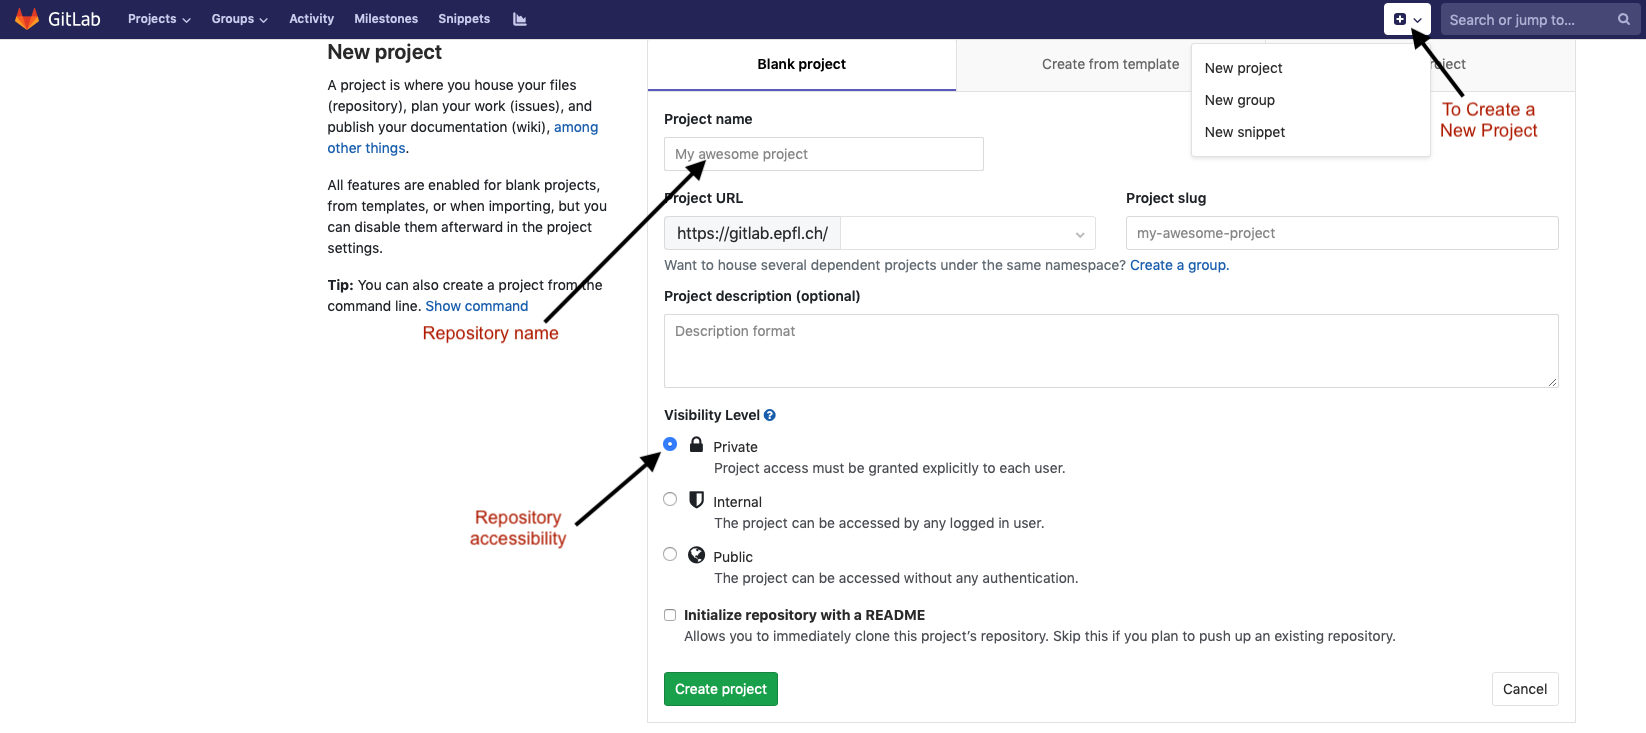
\includegraphics[width=\textwidth]{figures/GIT-RepositoryCreation}
  \caption{Creating a new git repository}
  \label{fig:git-create-repo}
\end{figure}

\subsection{Cloning}
\label{sec:personal-cloning}
The newly created repository can be cloned to your computer using the
same steps described earlier to clone the main exercise repository.

\begin{lstlisting}[language=bash]
$ git clone {REPOSITORY_CLONE_URL}
\end{lstlisting}

\subsection{Status}
\label{sec:personal-status}

One of the most important elements to keep track of your cloned
repository is to keep track of its status. You can do so at any time
by navigating in to the cloned repository on your terminal and then
executing the following command :

\begin{lstlisting}[language=bash]
$ git status
\end{lstlisting}

The output of the command will be explained in the following several
sub-sections.

\subsection{Pushing}
\label{sec:personal_push}

Once you have cloned the repository, you can now start populating your
cloned folder with the relevant files. GIT offers several stages in
maintaining your files:

\subsubsection{Stage 1 - Untracked files}
\label{sec:personal-untracked-files}

When new files is added for the first time to the cloned repository on
your computer, GIT recognizes the new files and add it under the
category of untracked files. Meaning GIT will not keep track of any
changes made to these files even though they are inside the
repository.

\subsubsection{Stage 2 - Tracked files}
\label{sec:stage-2-tracked}

One you decide a particular file needs to be tracked, you need to tell
GIT explicitly to do so. The command to do so is the following,

\begin{lstlisting}[language=bash]
$ git add {FILE}
\end{lstlisting}

The above command creates a snapshot of the file you are interested
in. This does NOT mean any changes you make after are kept track of,
when ever you think it is important to take a snapshot of the change
you made you need to execute this command on every file you are
interested in. This basically overwrites the previous snapshot you
made unless you committed the files.

\subsubsection{Stage 3 - Commit}
\label{sec:stage-3-commit}

Once you decided that a particular snapshot that you added
(one/several files) need to remembered as part of your history of
changes, you need to commit them.  You can commit your changes using
the command,

\begin{lstlisting}[language=bash]
$ git commit
\end{lstlisting}

This command will open up your default text editor from the
terminal. Here you are expected to write a short message describing
the changes you made to the files that you want keep in history. This
helps you later on to quickly look at your history messages in a
readable format to know the overview of changes made during different
stages of development. After you are done, the a snapshot of this
history is now saved on your computer locally.

\subsubsection{Stage 4 - Pushing}
\label{sec:stage-4-pushing}

Finally when you decide that the changes you made along with your history
should be seen by other members or needs to be stored on the cloud, you need
to push the history to the online repository using the command:

\begin{lstlisting}[language=bash]
$ git push
\end{lstlisting}

The first time you do this you have to tell GIT where you are trying to push the
changes using the command,

\begin{lstlisting}[language=bash]
$ git push --set-upstream origin master
\end{lstlisting}

Where,
origin represents that you are trying to push to the default online repository.
master represents the main branch of the repository that you are trying to push to.


\end{document}

%%% Local Variables:
%%% mode: latex
%%% TeX-master: t
%%% End:
